\documentclass[10pt,a4paper]{article}
\usepackage[utf8]{inputenc}
\usepackage{amsmath}
\usepackage{amsfonts}
\usepackage{amssymb}
\usepackage{graphicx}
\usepackage{hyperref}
\usepackage[normalem]{ulem}
\usepackage[left=2cm,right=2cm,top=2cm,bottom=2cm]{geometry}
\usepackage{array} 
%%%%%%%%%%%%%%%%%%%%%%%%%%%%%%%%%%%%%%%%%%%%%%%%%%%%%%%%%%%%%%
 % For code snippets
\usepackage{listings}
\usepackage{color}

\definecolor{dkgreen}{rgb}{0,0.6,0}
\definecolor{gray}{rgb}{0.5,0.5,0.5}
\definecolor{mauve}{rgb}{0.58,0,0.82}

\lstset{frame=tb,
  language=C,
  aboveskip=3mm,
  belowskip=3mm,
  showstringspaces=false,
  columns=flexible,
  basicstyle={\small\ttfamily},
  numbers=none,
  numberstyle=\tiny\color{gray},
  keywordstyle=\color{blue},
  commentstyle=\color{dkgreen},
  stringstyle=\color{mauve},
  breaklines=true,
  breakatwhitespace=true,
  tabsize=3
}
%%%%%%%%%%%%%%%%%%%%%%%%%%%%%%%%%%%%%%%%%%%%%%%%%%%%%%%%%%%%%%


%%%%%%%%%%%%%%%%%%%%%%%%%%%%%%%%%%%%%%%%%%%%%%%%%%%%%%%%%%%%%%%%%%%%%%%%%%%%%%%%%%%%%%%%%
% Declaring shapes that will be used when creating block diagrams using the tikz package%
%%%%%%%%%%%%%%%%%%%%%%%%%%%%%%%%%%%%%%%%%%%%%%%%%%%%%%%%%%%%%%%%%%%%%%%%%%%%%%%%%%%%%%%%%

\usepackage{tikz}
\usetikzlibrary{shapes.geometric, arrows, math}

\tikzstyle{camera} = [rectangle, rounded corners, minimum width=3cm, minimum height=1cm,text centered, draw=black, fill=red!30]

%%%%%%%%%%%%%%%%%%%%%%%%%%%%%%%%%%%%%%%%%%%%%%%%%%%%%%%%%%%%%%%%%%%%%%%%%%%%%%%%%%%%%%%%%

\title{RF Generator Software Architecture}

\begin{document}

%	\maketitle
%	\tableofcontents

	\begin{figure}
		\center
		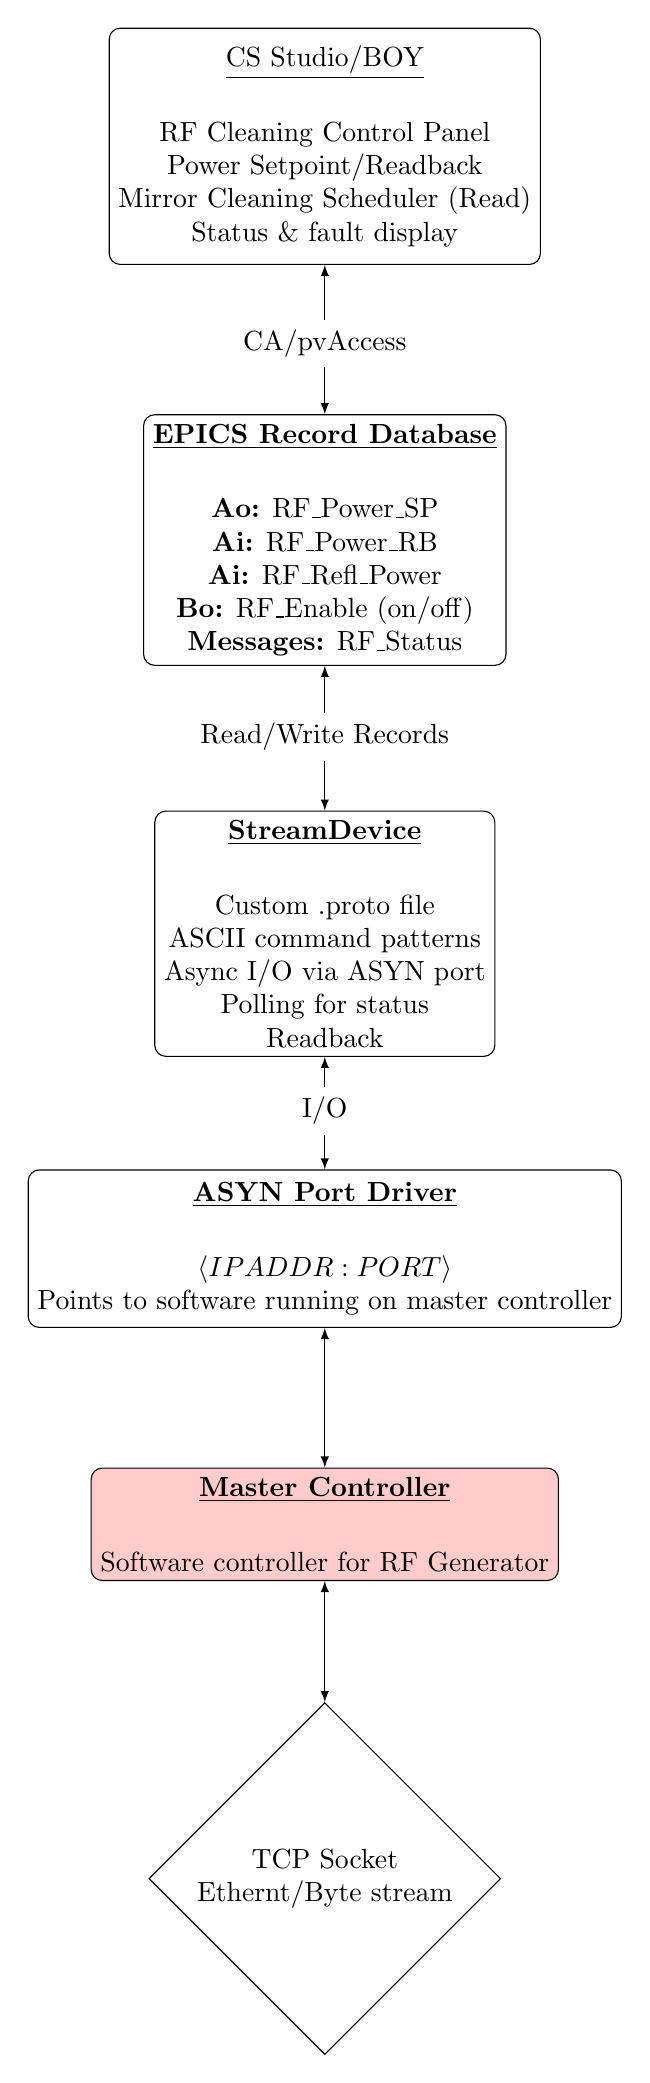
\begin{tikzpicture}
    \tikzmath{\xOpi = 0; \yOpi = 10; \yEpics = 5; \yStrm = 0; \yAsyn = -4; \yMaster = -7.5; \yEth = -12;}
    \node[align=center, minimum size=3cm, draw, rectangle, rounded corners](opi) at (\xOpi,\yOpi) {\underline{CS Studio/BOY}\\ \smallskip \\ RF Cleaning Control Panel\\ Power Setpoint/Readback\\ Mirror Cleaning Scheduler (Read)\\ Status \& fault display};

    \node[align=center, minimum size=3cm, draw, rectangle, rounded corners](epics-db) at (\xOpi,\yEpics) {\underline{\textbf{EPICS Record Database}}\\ \smallskip \\ \textbf{Ao:} RF\_Power\_SP \\ \textbf{Ai:} RF\_Power\_RB \\ \textbf{Ai:} RF\_Refl\_Power \\ \textbf{Bo:} RF\_Enable (on/off) \\ \textbf{Messages:} RF\_Status};

    \node[align=center](connect) at (\xOpi/2, \yEpics + \yOpi/2 - \yEpics/2){CA/pvAccess};

    \node[align=center, minimum size=3cm, draw, rectangle, rounded corners](strm-dev) at (\xOpi,\yStrm) {\underline{\textbf{StreamDevice}}\\ \smallskip \\ Custom .proto file \\ ASCII command patterns \\ Async I/O via ASYN port \\ Polling for status \\ Readback};

    \node[align=center](epics2strm-dev) at (\xOpi/2, \yStrm + \yEpics/2 - \yStrm/2){Read/Write Records};

    \node[align=center, minimum size=2cm, draw, rectangle, rounded corners](asyn-drv) at (\xOpi,\yAsyn) {\underline{\textbf{ASYN Port Driver}}\\ \smallskip \\ $\left\langle IP ADDR:PORT \right\rangle$ \\ Points to software running on master controller};

    \node[align=center](strm2asyn) at (\xOpi/2, \yAsyn + 1.75){I/O};

    \node[align=center, minimum size=1cm, draw, rectangle, rounded corners, fill=red!20](master-ctrl) at (\xOpi,\yMaster) {\underline{\textbf{Master Controller}}\\ \smallskip \\ Software controller for RF Generator};

    \node[align=center, minimum size=1cm, draw, diamond](eth-decis) at (\xOpi,\yEth) {TCP Socket \\ Ethernt/Byte stream};

    \draw[latex-] (opi) -- (connect);
    \draw[-latex] (connect) -- (epics-db);
    \draw[latex-] (epics-db) -- (epics2strm-dev);
    \draw[-latex] (epics2strm-dev) -- (strm-dev);
    \draw[latex-] (strm-dev) -- (strm2asyn);
    \draw[-latex] (strm2asyn) -- (asyn-drv);
    \draw[latex-latex] (asyn-drv) -- (master-ctrl);
    \draw[latex-latex] (master-ctrl) -- (eth-decis);
\end{tikzpicture}

%		\caption{adssaf}
		\label{fig:hdmi_tx_ss_flow_chart}
	\end{figure}

%	\newpage
	
	
%	\section{Overview of Beam Steering}
%	\label{sec:overview}
%		\input{src/bs_overview}	
%
%	\section{Beam Steering GUI}
%	\label{sec:bs_gui}
%		\input{src/bs_gui}
%
%	\section{Monitor Modes}
%	\label{sec:monitor_modes}
%		\input{src/monitor_modes}
%	
%	\section{HDMI\_ILock Sub-Block}
%	\label{sec:hdmi_ilock}
%		\input{src/hdmi_ilock}
%	
%	\section{Digilent rgb2dvi}
%	\label{sec:rgb2dvi}
%		\input{src/rgb2dvi}
%		
%	\section{lwip Problems}
%	\label{sec:lwip_problems}
%		\input{src/lwip_problems}
		
%	\section{HDMI 1.4/2.0 Transmitter Subsystem}
%	\label{sec:hdmi_tx_ss}
%		\input{src/hdmi_tx_ss}

%	\newpage
	
%	\section{FPGA Video Interfacing Notes}
%	\label{sec:fpga_vid_interfac}
%		\input{src/fpga_video_interface_notes}

%	\section{Current Project Details}
%	\label{sec:cur_prj_dets}
%		\input{src/bs_prj_specs}
		
%	\section{Configuring zcu102 Board to Work with Sundance FMC Card}
%	\label{sec:config_zcu102_for_sundance}
%		\input{src/config_zcu102_for_sundance_fmc}
%	
%	\section{Project Descriptions}
%	\label{sec:proj_descript}
%		\input{src/bs_project_descriptions}
%	
%	\section{Evaluation License for HDMI 1.4/2.0 Transmitter Subsystem IP}
%	\label{sec:eval_license_hdim_tx_ss}
%		\input{src/eval_license_hdim_tx_ss}
%	
%	\section{Server Control Commands}
%	\label{sec:serv_ctrl_cmds}
%		\input{src/server_ctrl_comands}
%	
%	\section{BWS Quick Tune}
%	\label{sec:bws_quick_tune}
%		\input{src/bws_quick_tune}
%	
%	\section{Build Python UI for Distribution}
%	\label{sec:build_python_ui_for_dist}
%		\input{src/build_python_ui_for_distribution}
%	
%	\section{FDAC}
%	\label{sec:fdac}
%		\input{src/FSMCtrl_IP_rewrite}
%		
%	\newpage	
%	
%	\section{Working Notes}
%	\label{sec:working_notes}
%		\input{src/bs_working_notes}
		
\end{document}